% !TeX root = text.tex
\chapter{hardware}

\section{Raspberry Pi}

\section{Galvanometr a zrcátko}
\begin{itemize}
  \item
        Galvanometry, často nazývané galva, jsou elektronické součástky používané k měření intenzity a směru elektrického proudu.~\cite{galvo}

        Můžeme je rozdělit mezi galvanometry s uzavřenou smyčkou zpětné vazby (CLGS) a galvanometry bez uzavřené smyčky zpětné vazby (OLGS).~\cite{how-ls-work}
        % Druhé zmíňěné mají velice specifické využití - barcode scanners a jsou zdokumentované pouze ve zdroji .

        \cite{advanced-galvo}
        ale postupně nachází uplatnění ve více a více odvětvích práce s lasery.
        Oproti jiným možnostem nabízí flexibilitu, rychlost a přesnost za nízkou cenu.


        V této práci jsou ale využívány CLGS, které jsou lépe zdokumentované.

        V CLGS jsou potřeba 3 hlavní prvky, %pohybový akční člen, senzor a kontrolní desku - vycucáno z prstu

        Nejmodernější galvanometrové polohovací systémy jsou založené na principech elektromotorů s permanentními magnety, kde
        \cite{advanced-galvo}
  \item
        \url{https://en.wikipedia.org/wiki/Galvanometer}\\
        \url{https://en.wikipedia.org/wiki/Laser_scanning}\\
        \url{https://en.wikipedia.org/wiki/Mirror_galvanometer}\\
        \url{https://en.wikipedia.org/wiki/Laser_lighting_display}

        A mirror galvanometer is an ammeter that indicates it has sensed an electric current by deflecting a light beam with a mirror.
        The mirror galvanometer consists of a long fine coil of silk-covered copper wire. %wtf silk == hedvábí??
        In the heart of that coil, within a little air-chamber, a small round mirror is hung by a single fibre of floss silk, with four tiny magnets cemented to its back
        The small weight of the mirror and magnets which form the moving part of this instrument, and the range to which the minute motions of the mirror can be magnified on the screen by the reflected beam of light, which acts as a long impalpable hand or pointer, render the mirror galvanometer marvellously sensitive to the current, especially when compared with other forms of receiving instruments.

        Zrcadlový galvanometr je měřič proudu, který reaguje na měřený proud vychýlením světelného paprsku zrcátkem připevněném na jeho konci.
        % Skládá se z dlouhé  tenké cívky měděného drátu potaženého hedvábím %wtf silk == hedvábí??
        % Ve středu této cívky je v malé vzduchové komůrce na jediném vláknu hedvábí

        Skládá se z cívky a
        \cite{zrcadlovy-galvanometr-wiki}

  \item
        \bardgen{2023-10-20}{popiš mi jak je sestaven a jak funguje galvanometr se zrcátkem k odrážení světelného paprsku}{
          Galvanometr se zrcátkem je sestaven z následujících komponent:

          * **Cívka:** Cívka je navinuta na jádře z feromagnetického materiálu, jako je železo nebo nikl. Cívkou prochází elektrický proud, který vytváří magnetické pole.
          * **Ukazatel:** Ukazatel je připojen k cívce a je vyroben z lehkého materiálu, jako je hliník nebo plast. Ukazatel je vychýlen magnetickým polem vytvářeným cívkou.
          * **Zrcátko:** Zrcátko je připojeno k ukazateli a odráží světelný paprsek.
          * **Okulár:** Okulár je umístěn tak, aby bylo možné pozorovat odraz světelného paprsku.

          **Jak funguje:**

          Když prochází cívkou elektrický proud, vytváří magnetické pole. Toto magnetické pole působí na ukazatel a vychýlí ho. Velikost výchylky ukazatele je přímo úměrná velikosti proudu procházejícího cívkou.

          Zrcátko je připojeno k ukazateli a odráží světelný paprsek. Když se ukazatel vychýlí, odraz světelného paprsku se také vychýlí.

          Okulár je umístěn tak, aby bylo možné pozorovat odraz světelného paprsku. Velikost vychýlení světelného paprsku je přímo úměrná velikosti proudu procházejícího cívkou.

          **Výhody:**

          * Galvanometr se zrcátkem je citlivější než galvanometr bez zrcátka.
          * Galvanometr se zrcátkem lze použít k měření velmi malých proudů.

          **Nevýhody:**

          * Galvanometr se zrcátkem je dražší než galvanometr bez zrcátka.

          **Použití:**

          Galvanometr se zrcátkem se používá k měření velmi malých proudů. Používá se například v elektrotechnice, lékařství a fyzice.
        }
\end{itemize}

ovládá se variabilním proudem

\section{hlavice}
\href{https://elenlaser.com/blog/galvo-head-laser-focus-tool.html}{The mirrors, mounted perpendicularly on the engines, move the laser beam along the X and Y axes according to the input received from the motor.
The big advantage of these devices is that they can reach a very high acceleration and speed of}
well asi patří do sekce galvanometr

\section{moje deska na napětí}
Galvanometry v obou osách pohybu potřebujeí analogový vstupní signál v rozpětí $-15$~V až $+15$~V udávající vychýlení galvanometru v daném směru.

Obvod, který se stará o vytváření tohoto signálu je založený na obvodu ze zdroje \cite{lasershow-with-real-galvos}.
Vytváření tohoto signálu je rozděleno do dvou částí. Nejdříve DAC (digital-to-analog converter, D/A převodník) připojený k RPi vytvoří signál v rozpětí 0 až 5~V a následně je tento signál pomocí operačního zesilovače převeden na požadované rozpětí, tj. $-15$~V až $+15$~V.
Jednotlivé části tohoto obvodu jsou blíže popsány v následujících kapitolách. Celé zapojení je vidět na obrázku \ref{fig:dac_board}.
\fxnote{unreadable text, make schem more compact}
\begin{figure}[!htb]
  \centering
  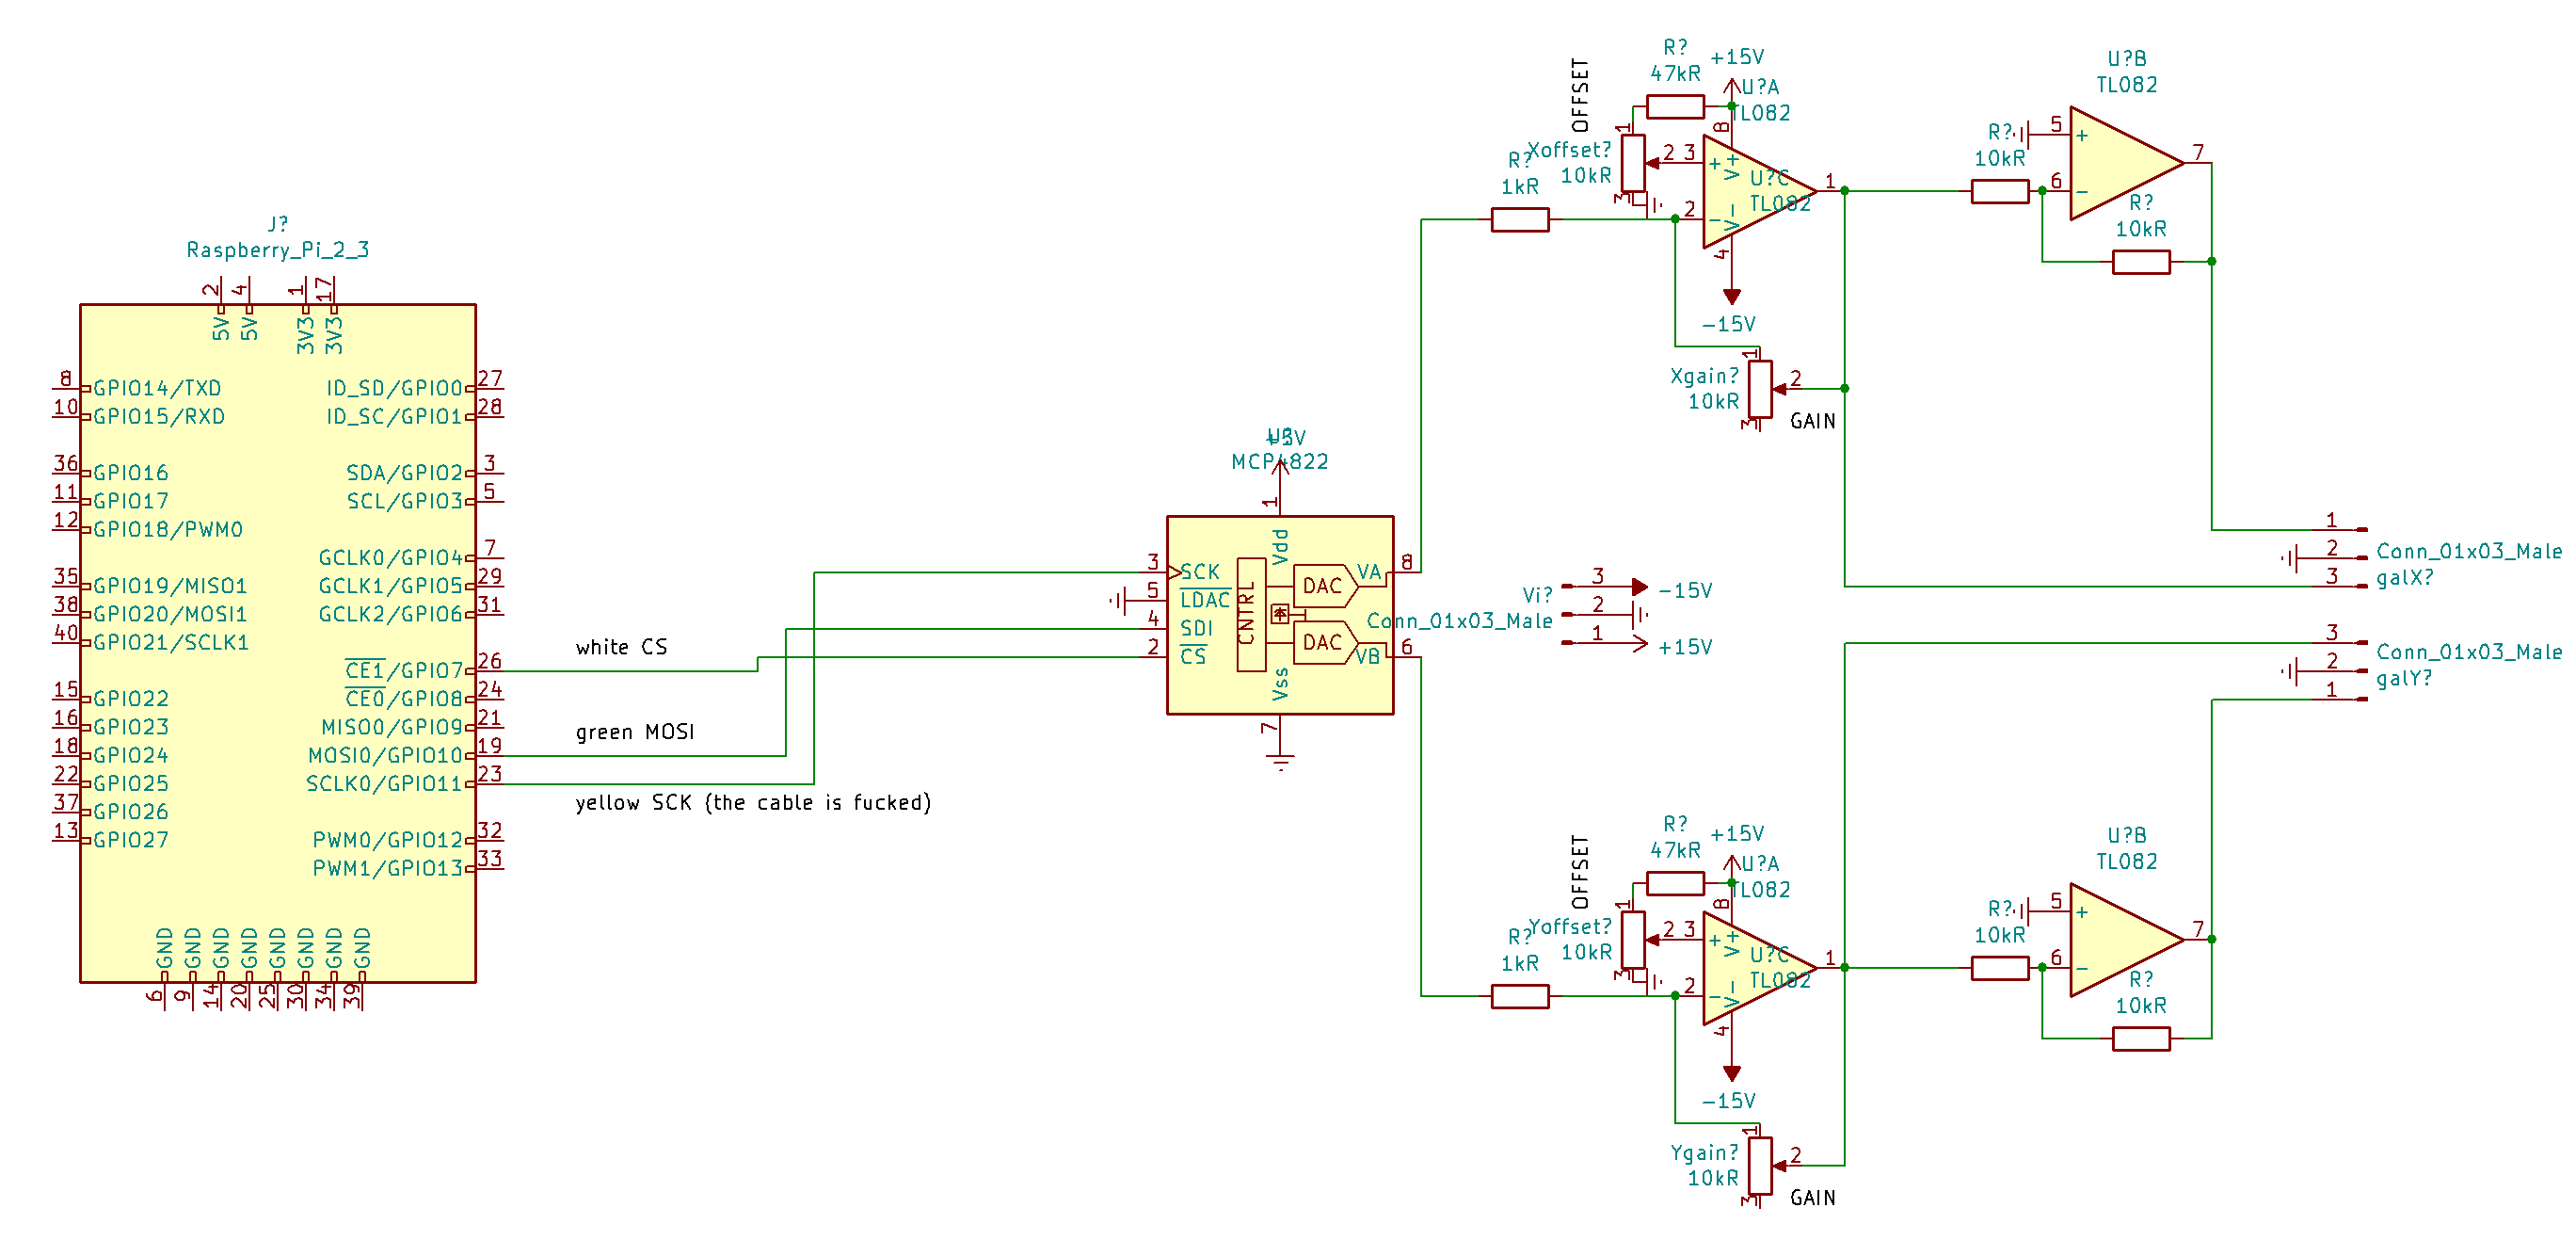
\includegraphics[width=1\textwidth]{img/dac_board.png} 
  \caption{\label{fig:dac_board}Zapojení DAC a zesilovačů k RPi a řídící desce galvanometrů}
\end{figure}

\subsection{dac}
K generování signálu v rozpětí 0--5~V jsem využil DAC MCP4822 od firmy \href{https://www.microchip.com}{Microchip Technology Inc.}\ \fxnote{TODO tečka? ("\textbackslash " == explicitni mezera)}
Tento čip podporuje komunikaci přes rozhraní SPI, pracuje s napájecím napětím 5~V a s 12bitovým rozlišením (je schopen vygenerovat 4~096 různých napětí) na dvou kanálech.

RPi komunikuje s čipem pomocí rozhraním SPI, toto rozhraní využívám pomocí knihovny ze serveru \url{https://github.com}\footnote{\url{https://github.com/abelectronicsuk/ABElectronics_CPP_Libraries/tree/master/ADCDACPi}; staženo 2.~1.~2024} \fxnote{TODO tečka?}
\fxnote{TODO more spec}
Tato knihovna poskytuje následující funkce, se kterými pracuji v mém kódu.
\begin{itemize}
\item
\lstinline[language=C]!bool mcp4822_initialize();!
\item
\lstinline[language=C]!bool mcp4822_set_voltage(mcp4822_channel_t channel, uint16_t value_mV);!
\item
\lstinline[language=C]!void mcp4822_deinitialize();!
\end{itemize}
\subsection{amps}
K rozšíření signálu z DAC jsem využil dva operační zesilovače TL082 od firmy \href{https://www.ti.com/}{Texas Instruments Incorporated}. Každý z nich je připojený na jeden kanál DAC čipu mcp4822.
\fxnote{TODO more spec}
Tyto čipy mi napěťové rozpětí zvýší z 0--5~V na $-15$~V až $+15$~V.

zesilovac - cteni baterek \url{https://is.muni.cz/el/sci/jaro2017/F5090/um/E17_P8.pdf}

\section{laser}
\section{if rgb: 3 dacs}


\fxnote{TODO cos udelal svyho vlastne a jak to facha}

\section{napájení}
\fxnote{TODO ay tak co, zvladls to dat na baterky?}
